% =====================================================================
% 第 6 章  实验与分析  (Chapter 6 draft)
% 配套图表已生成于 Temperature_predictor/figures/
% 配套实验数据位于 Temperature_predictor/experiments/
% 请按学校论文模板调整字体/章节命令 (\chapter / \section / 中文标题等)
% =====================================================================

\chapter{实验与分析}
\label{ch:experiment}

本章在第~\ref{ch:dataset}~章构建的数据集与第~\ref{ch:graph}--\ref{ch:model}~章提出的先验图--AGCRN 模型基础上，系统评估所提方法在中-长期海温异常预测任务上的性能。
\ref{sec:exp:setup}~节给出实验设置；\ref{sec:exp:baseline}~节给出与传统方法的整体对比；\ref{sec:exp:main}~节分析主模型的训练过程与时空误差结构；\ref{sec:exp:ablation}~节通过对图融合权重 $\lambda$ 的消融研究讨论先验图与自适应图各自的作用；\ref{sec:exp:discussion}~节对实验结果进行综合讨论并指出当前模型的局限。

% ---------------------------------------------------------------------
\section{实验设置}
\label{sec:exp:setup}

\subsection{数据划分}
依照第~\ref{ch:dataset}~章所述，研究区域为 $120^{\circ}$E--$280^{\circ}$E、$30^{\circ}$S--$30^{\circ}$N，2$^{\circ}$ 网格下共 $H\!\times\!W=30\!\times\!80$ 个像素，其中海洋节点 $N=2276$。时间范围为 2015--2024 年共 $T=3639$ 天。在时间维度按 7\!:\!1\!:\!2 划分：训练集 2015-01-01 -- 2021-12-31（2544 天）、验证集 2022 年（365 天）、测试集 2023--2024 年（730 天）。在 $(T_{\text{in}}, T_{\text{out}}) = (30, 30)$ 的滑窗采样下，三集分别得到 2485 / 306 / 671 个独立样本，所有窗口完全包含于其所属时段，避免跨集泄露。

\subsection{评价指标}
对每个 lead 天数 $\ell\in\{1,\ldots,30\}$，分别计算下列指标（$\hat y, y$ 已反归一化为海温异常 $^{\circ}$C）：
\begin{align}
\text{RMSE}(\ell) &= \sqrt{\tfrac{1}{N}\sum_{i=1}^{N}(\hat y_{\ell,i}-y_{\ell,i})^2}, \\
\text{MAE}(\ell)  &= \tfrac{1}{N}\sum_{i=1}^{N}|\hat y_{\ell,i}-y_{\ell,i}|, \\
r(\ell) &= \mathrm{Corr}(\hat y_{\ell,\cdot},\, y_{\ell,\cdot}), \\
\text{SSIM}(\ell) &= \mathrm{SSIM}(\mathrm{Grid}(\hat y_\ell),\,\mathrm{Grid}(y_\ell)),
\end{align}
其中 $\mathrm{Grid}(\cdot)$ 将 $N$ 维海洋向量按掩膜还原为 $H\!\times\!W$ 二维场后送入标准 SSIM 实现 \citep{wang2004ssim}。RMSE/MAE 越低越好，$r$/SSIM 越高越好。报告时重点关注 $\ell\in\{1, 7, 14, 30\}$ 四个代表性 lead。

\subsection{基线方法}
为定位 AGCRN 在 SST 异常预测任务上的相对水平，引入两类无可学习参数的物理-气候基线：
\begin{itemize}
    \item \textbf{Persistence}：取输入窗口最后一日的 SSTA 作为未来 30 天的常值预测，刻画"短期海温场具有强惰性"这一物理事实。
    \item \textbf{Climatology}：以训练集 2015--2021 年的逐日多年气候态平均作为预测，对应"无任何动力信息"的零信息基准。由于工作变量为 SST \emph{异常}，理论上其期望值为 0；该基线衡量的是模型相对"什么都不预测"的提升量。
\end{itemize}

\subsection{超参与硬件}
所有 AGCRN 训练共享下表~\ref{tab:hyper}~所列超参，并使用 Adam 优化器、L1 损失、梯度裁剪 $5.0$、学习率 $10^{-3}$；早停 patience 为 15。云端使用 NVIDIA RTX 5090 (32\,GB, sm\_120) 配合 PyTorch 2.7+cu128，训练时启用混合精度 (AMP) 与 30 步时序梯度检查点；单次 25-epoch 训练耗时约 43 分钟，模型可学习参数 0.79\,M。

\begin{table}[ht]
\centering
\caption{AGCRN 主模型超参}
\label{tab:hyper}
\begin{tabular}{ll|ll}
\hline
窗口长度 $T_\text{in}$ & 30 & 隐藏维度 $h$ & 64 \\
预测长度 $T_\text{out}$ & 30 & 层数 $L$ & 2 \\
节点嵌入 $d_E$ & 10 & 切比雪夫阶 $K$ & 2 \\
自适应嵌入 $d_a$ & 10 & 融合权重 $\lambda$ & 0.5 (默认) \\
批大小 & 32 / 64 & 训练轮数 & 100 (早停) \\
\hline
\end{tabular}
\end{table}

% ---------------------------------------------------------------------
\section{与基线方法的整体比较}
\label{sec:exp:baseline}

表~\ref{tab:baseline}~给出 AGCRN 主模型 (seed = 42, $\lambda=0.5$) 与两个基线在 4 个代表性 lead 上的测试集结果，图~\ref{fig:lead_decay_baseline}~呈现完整 30 天的衰减曲线。

\begin{table}[ht]
\centering
\caption{测试集上 AGCRN 与基线方法的性能对比 (RMSE 与 MAE 单位 $^{\circ}$C)。粗体表示该 lead 上的最佳值。}
\label{tab:baseline}
\small
\begin{tabular}{l|cccc|cccc}
\hline
\multirow{2}{*}{Method} & \multicolumn{4}{c|}{RMSE $\downarrow$} & \multicolumn{4}{c}{Pearson $r$ $\uparrow$} \\
                        & 1d & 7d & 14d & 30d & 1d & 7d & 14d & 30d \\
\hline
Persistence  & \textbf{0.205} & 0.614 & 0.794 & 0.948 & 0.776 & 0.038 & $-0.117$ & $-0.029$ \\
Climatology  & 1.121 & 1.121 & 1.123 & 1.124 & $-0.001$ & $-0.001$ & $-0.001$ & $-0.001$ \\
AGCRN (ours) & 0.210 & \textbf{0.578} & \textbf{0.709} & \textbf{0.807} & \textbf{0.873} & \textbf{0.163} & $-0.086$ & $-0.018$ \\
\hline
\end{tabular}
\end{table}

\begin{figure}[ht]
\centering
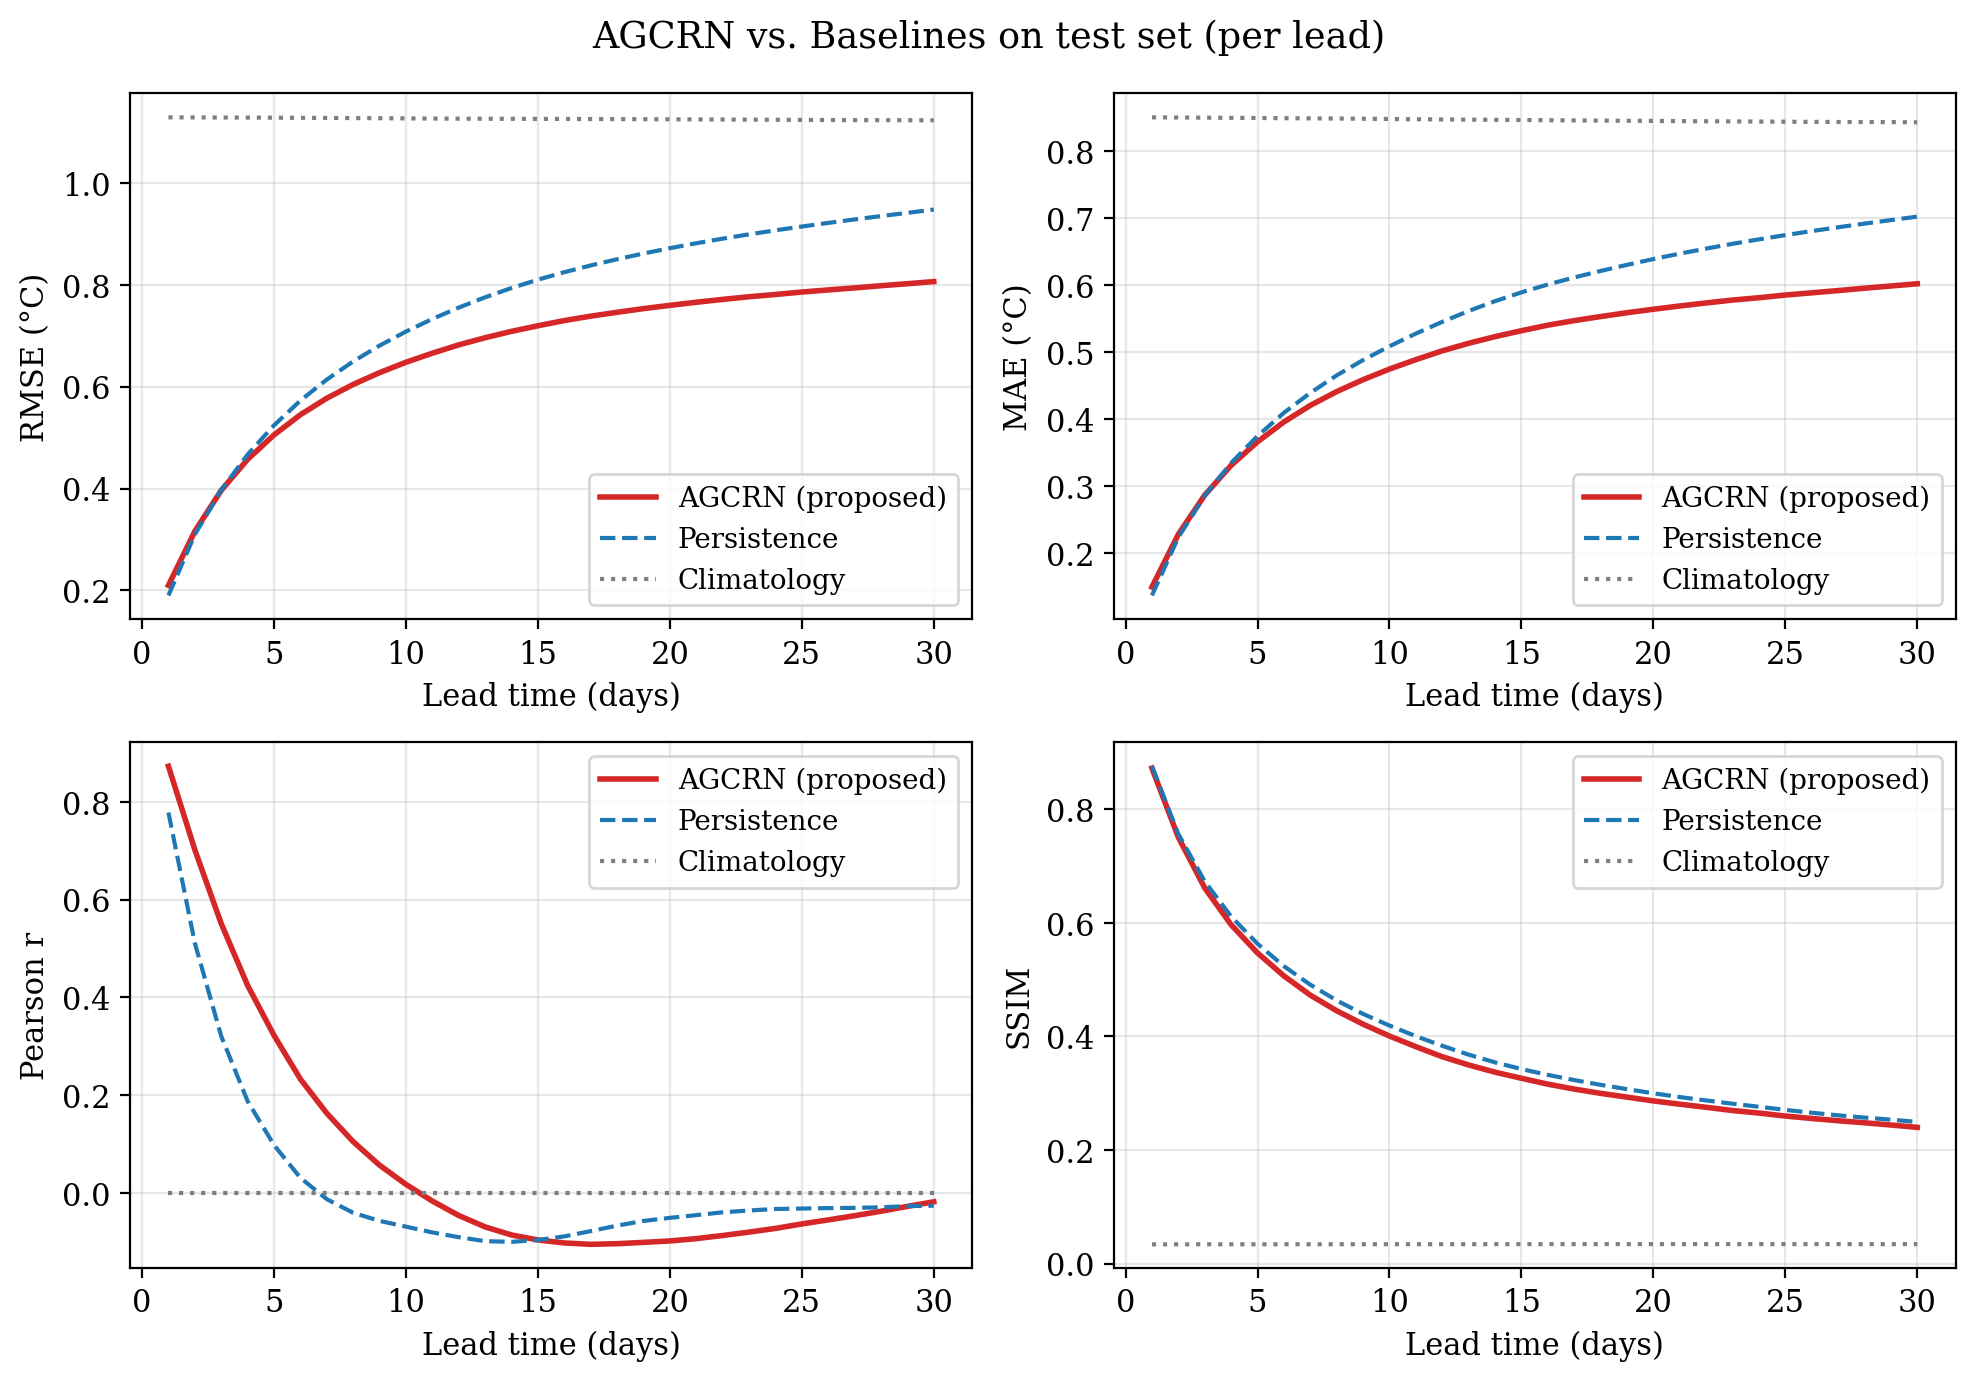
\includegraphics[width=0.95\linewidth]{figures/fig_lead_decay_baseline.png}
\caption{AGCRN 与 Persistence、Climatology 在测试集上的逐 lead 指标曲线。AGCRN 在 RMSE/MAE/Pearson 三项上从 lead $\ge\!2$ 起即明显优于 Persistence；Climatology 给出常值参考。}
\label{fig:lead_decay_baseline}
\end{figure}

\paragraph{观察与解释}
\begin{itemize}
    \item \textbf{短期 (1\,d)}：AGCRN 与 Persistence 数值接近 (RMSE 0.210 vs 0.205)，反映 SSTA 在 1 天尺度上由强自相关主导，几乎不需"建模"——这与海洋热惯性的物理事实一致。
    \item \textbf{中期 (7\,--\,14\,d)}：AGCRN 取得最显著优势，在 7 天和 14 天 lead 上 RMSE 分别较 Persistence 降低 $5.9\%$ 和 $10.7\%$；Pearson $r$ 由 Persistence 的 $0.038$ 提升至 $0.163$，表明所学时空动力捕获了仅靠"维持现状"无法描述的演化信号。
    \item \textbf{长期 (30\,d)}：AGCRN 的 RMSE 较 Persistence 降低 $14.9\%$ 至 $0.807\,^{\circ}$C，但所有方法 Pearson 均落入 $[-0.1, 0]$ 区间。这是 SSTA 任务在 30 天尺度本征不可预测性的体现：异常信号已被大尺度内部变率吞没。AGCRN 在该尺度上的优势主要体现在"幅值控制"(RMSE/MAE) 而非"形状对齐"($r$/SSIM)。
    \item Climatology 在异常域上恒为 0，因此 RMSE 接近 SSTA 的标准差 ($\approx 1.12\,^{\circ}$C)，构成所有方法理应突破的下限。AGCRN 相对 Climatology 在 30 天 lead 上仍能降低 $28.2\%$，证明可学习时空模型对"远期均值预测"也能贡献信息。
\end{itemize}

% ---------------------------------------------------------------------
\section{主模型详细分析}
\label{sec:exp:main}

\subsection{训练过程}
图~\ref{fig:train_curves}~展示主模型的训练损失与验证 RMSE 随 epoch 的演化曲线。模型在第 7--10 epoch 取得验证集最优，此后验证 RMSE 出现轻微回升，触发 patience=15 早停 (实际终止于 epoch 25)。最优验证集 RMSE 为 $0.6637\,^{\circ}$C。训练损失持续下降而验证集不再改善，表明 0.79\,M 参数的网络在 2485 个训练样本上的容量已达饱和；这一现象在 \ref{sec:exp:ablation}~节关于自适应图分支的讨论中将进一步呈现。

\begin{figure}[ht]
\centering
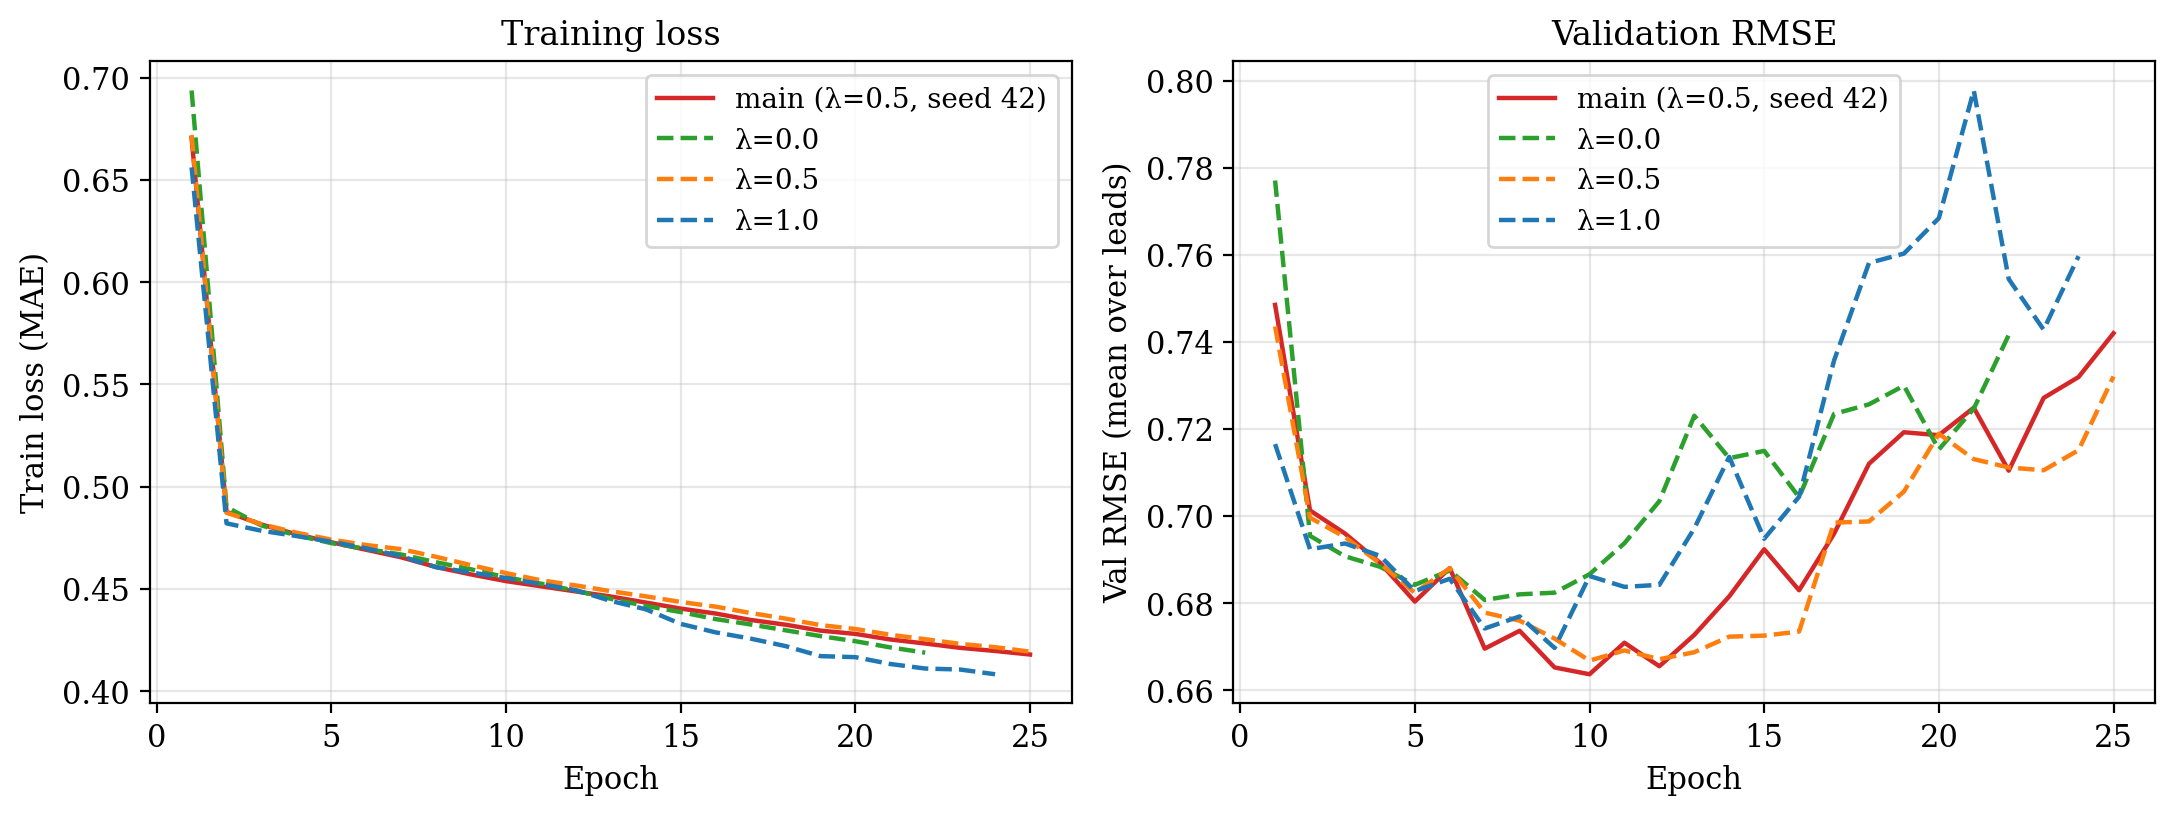
\includegraphics[width=0.95\linewidth]{figures/fig_train_curves.png}
\caption{AGCRN 主模型与三组 $\lambda$-消融实验的训练损失 (左) 与验证 RMSE (右)。所有曲线在 7--10 轮即触及验证最优。}
\label{fig:train_curves}
\end{figure}

\subsection{逐像素空间误差}
图~\ref{fig:spatial_rmse}~展示主模型在测试集所有样本上、4 个代表性 lead 处的逐像素 RMSE 空间分布。相比表~\ref{tab:baseline}~给出的"先空间平均、再时间平均"标量，逐像素 RMSE 更能揭示模型在不同物理过程主导区域的能力差异。
\begin{figure}[ht]
\centering
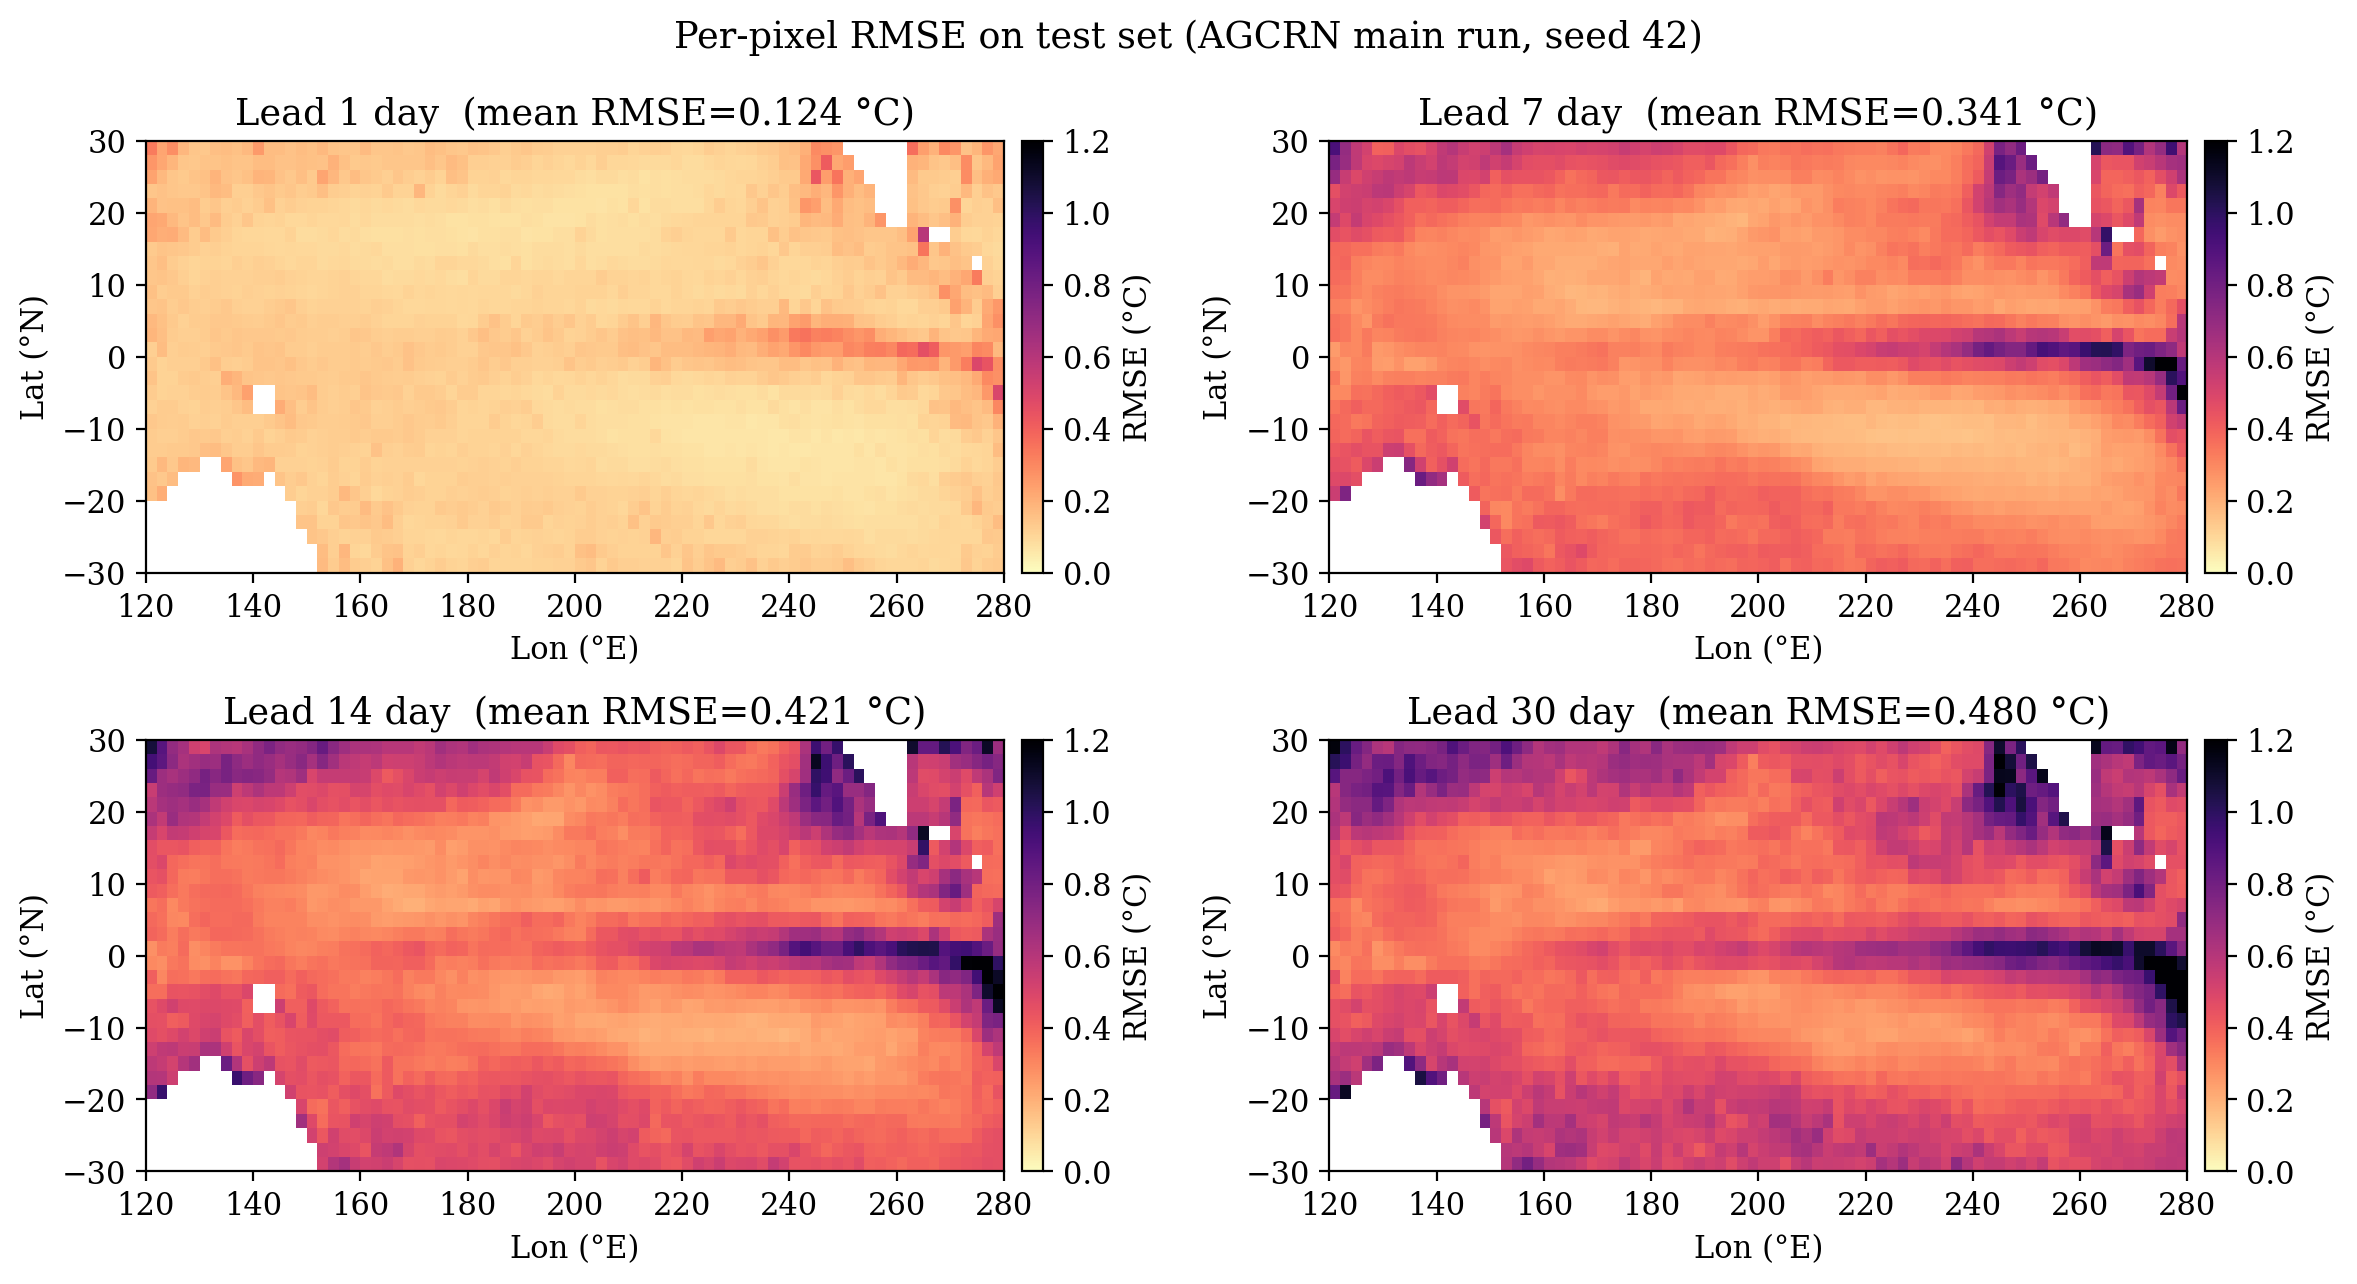
\includegraphics[width=0.95\linewidth]{figures/fig_spatial_rmse.png}
\caption{AGCRN 主模型在测试集上的逐像素 RMSE 空间分布 ($^{\circ}$C)。}
\label{fig:spatial_rmse}
\end{figure}

\paragraph{结构性误差}三个特征显著：
\begin{enumerate}
    \item \textbf{赤道带的高误差走廊}：在 $\sim\!0^{\circ}$N、$160^{\circ}$E\,--\,$270^{\circ}$E 一线 RMSE 系统性偏大，对应 ENSO 海温异常活跃区。该区域 SST 受 Bjerknes 反馈与 Kelvin/Rossby 波传播控制，演化的非平稳性强、内部变率大，对仅以 30 天历史窗为输入的纯数据驱动模型构成天然挑战。
    \item \textbf{北半球副热带与中纬误差带}：$\sim\!20^{\circ}$N\,--\,$30^{\circ}$N 的西北太平洋及加州沿岸表现出次显著的高 RMSE 区，对应黑潮、加州冷流等强西边界流/上升流系统，存在中尺度涡旋与锋面，2$^{\circ}$ 粗网格无法分辨这些次网格过程，导致模型本征系统误差。
    \item \textbf{中央太平洋低误差洼地}：$5^{\circ}$S\,--\,$15^{\circ}$N 中部洋面 RMSE 始终保持在 $0.3\,^{\circ}$C 以下，因该区域以风驱动的稳定大尺度环流为主，SST 平流-扩散主导，先验距离图能很好刻画其局部结构。
\end{enumerate}

\subsection{个例分析}
图~\ref{fig:case_study}~展示测试集第 200 号样本（对应 2024 年中某 30 天预测窗）在 4 个 lead 上的真值、预测与误差三联图。
\begin{figure}[ht]
\centering
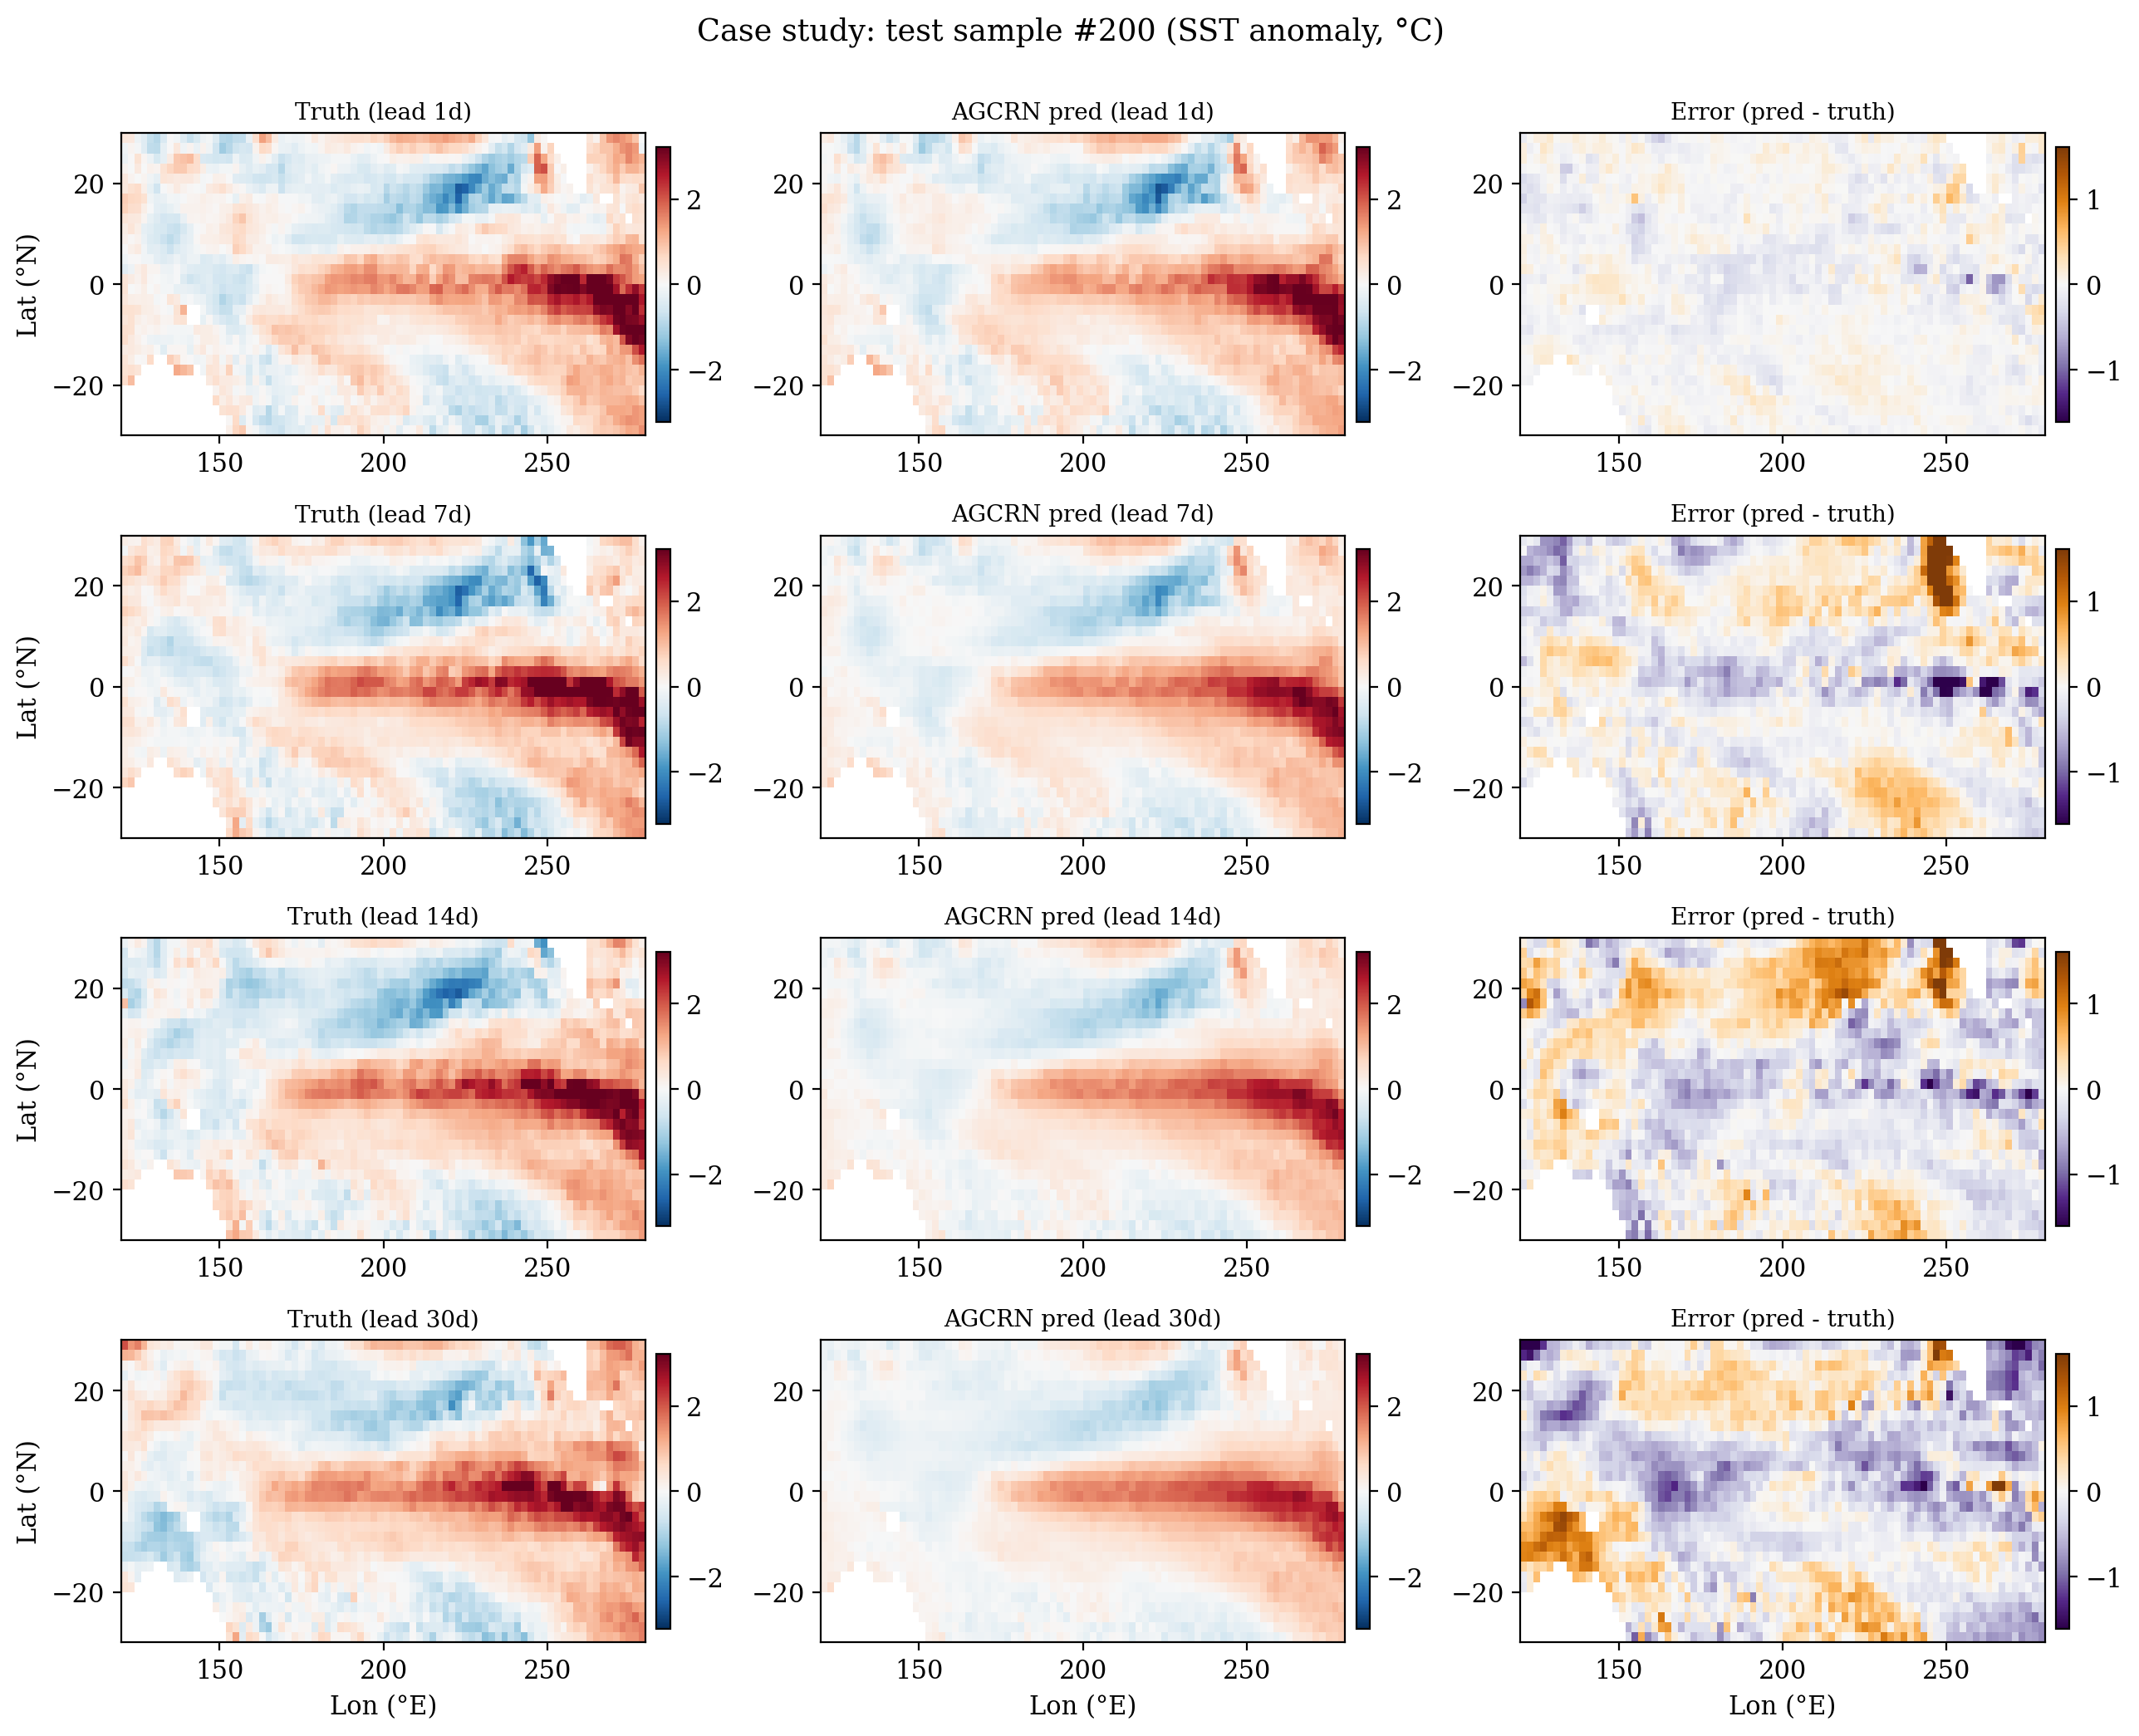
\includegraphics[width=0.95\linewidth]{figures/fig_case_study.png}
\caption{测试样本 \#200 的真值、AGCRN 预测与逐像素误差。颜色域为 SST 异常 ($^{\circ}$C)。}
\label{fig:case_study}
\end{figure}

\begin{itemize}
    \item lead = 1\,d 时预测与真值几乎重合 (右列误差 $\le\!0.3\,^{\circ}$C)，模型有效捕获了该样本所对应的赤道东太平洋暖异常带。
    \item lead = 7\,d 起，赤道东太平洋暖异常出现幅值低估 (中列同位置颜色变浅)，西北太平洋的冷异常涡旋则因模型的空间平滑而被"抹去"，转化为右列对应区域的正误差。
    \item lead = 30\,d 时预测仍保留正确的"赤道暖--副热带冷"宏观格局，但幅值进一步衰减；这与 \ref{sec:exp:baseline}~节观察到的"长期 RMSE 主要由幅值压缩贡献"一致。
\end{itemize}
该个例直观地反映出当前模型的两类典型失败模式：(i) 中尺度结构在长 lead 上的耗散，(ii) 强信号 (如 ENSO 暖区) 的幅值低估。

% ---------------------------------------------------------------------
\section{图融合权重的消融研究}
\label{sec:exp:ablation}

为厘清先验图与自适应图各自的贡献，固定其它超参不变，仅扫描融合权重 $\lambda \in \{0.0, 0.5, 1.0\}$ 训练三组模型。$\lambda = 0$ 对应"纯自适应图"(Bai 等 2020 原版 AGCRN)，$\lambda = 1$ 对应"纯先验图"(无自适应分支)，$\lambda = 0.5$ 对应等权融合。表~\ref{tab:ablation}~汇总测试集结果，图~\ref{fig:ablation_bar}~与图~\ref{fig:lead_decay_ablation}~分别给出柱状对比与全 lead 衰减曲线。

\begin{table}[ht]
\centering
\caption{$\lambda$-融合权重消融。粗体为该 lead 最佳。RMSE/MAE 单位 $^{\circ}$C。}
\label{tab:ablation}
\small
\begin{tabular}{l|c|cccc|cccc}
\hline
\multirow{2}{*}{Config} & \multirow{2}{*}{val\_RMSE} & \multicolumn{4}{c|}{Test RMSE $\downarrow$} & \multicolumn{4}{c}{Test SSIM $\uparrow$} \\
        &       & 1d & 7d & 14d & 30d & 1d & 7d & 14d & 30d \\
\hline
$\lambda=0.0$ (pure adaptive)  & 0.6807 & 0.339 & 0.612 & 0.729 & 0.827 & 0.747 & 0.448 & 0.326 & 0.229 \\
$\lambda=0.5$ (fusion)         & \textbf{0.6668} & 0.238 & 0.583 & 0.712 & 0.812 & 0.848 & 0.468 & 0.337 & 0.239 \\
$\lambda=1.0$ (pure prior)     & 0.6697 & \textbf{0.228} & \textbf{0.578} & \textbf{0.705} & \textbf{0.801} & \textbf{0.856} & \textbf{0.470} & \textbf{0.340} & \textbf{0.246} \\
\hline
\end{tabular}
\end{table}

\begin{figure}[ht]
\centering
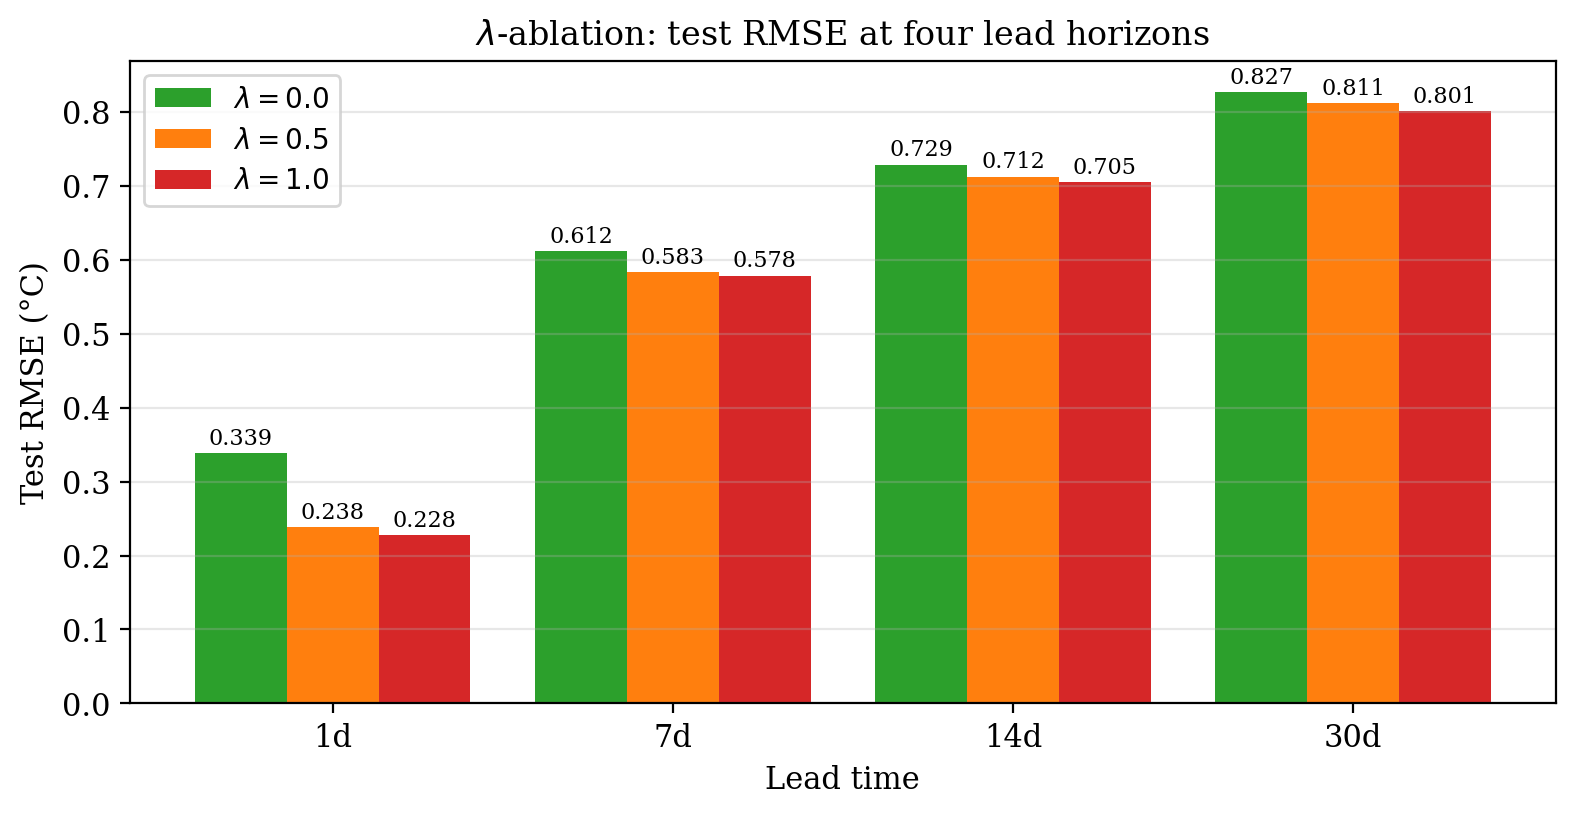
\includegraphics[width=0.85\linewidth]{figures/fig_ablation_bar.png}
\caption{$\lambda$ 消融实验：四个代表性 lead 上的测试 RMSE 柱状图。}
\label{fig:ablation_bar}
\end{figure}

\begin{figure}[ht]
\centering
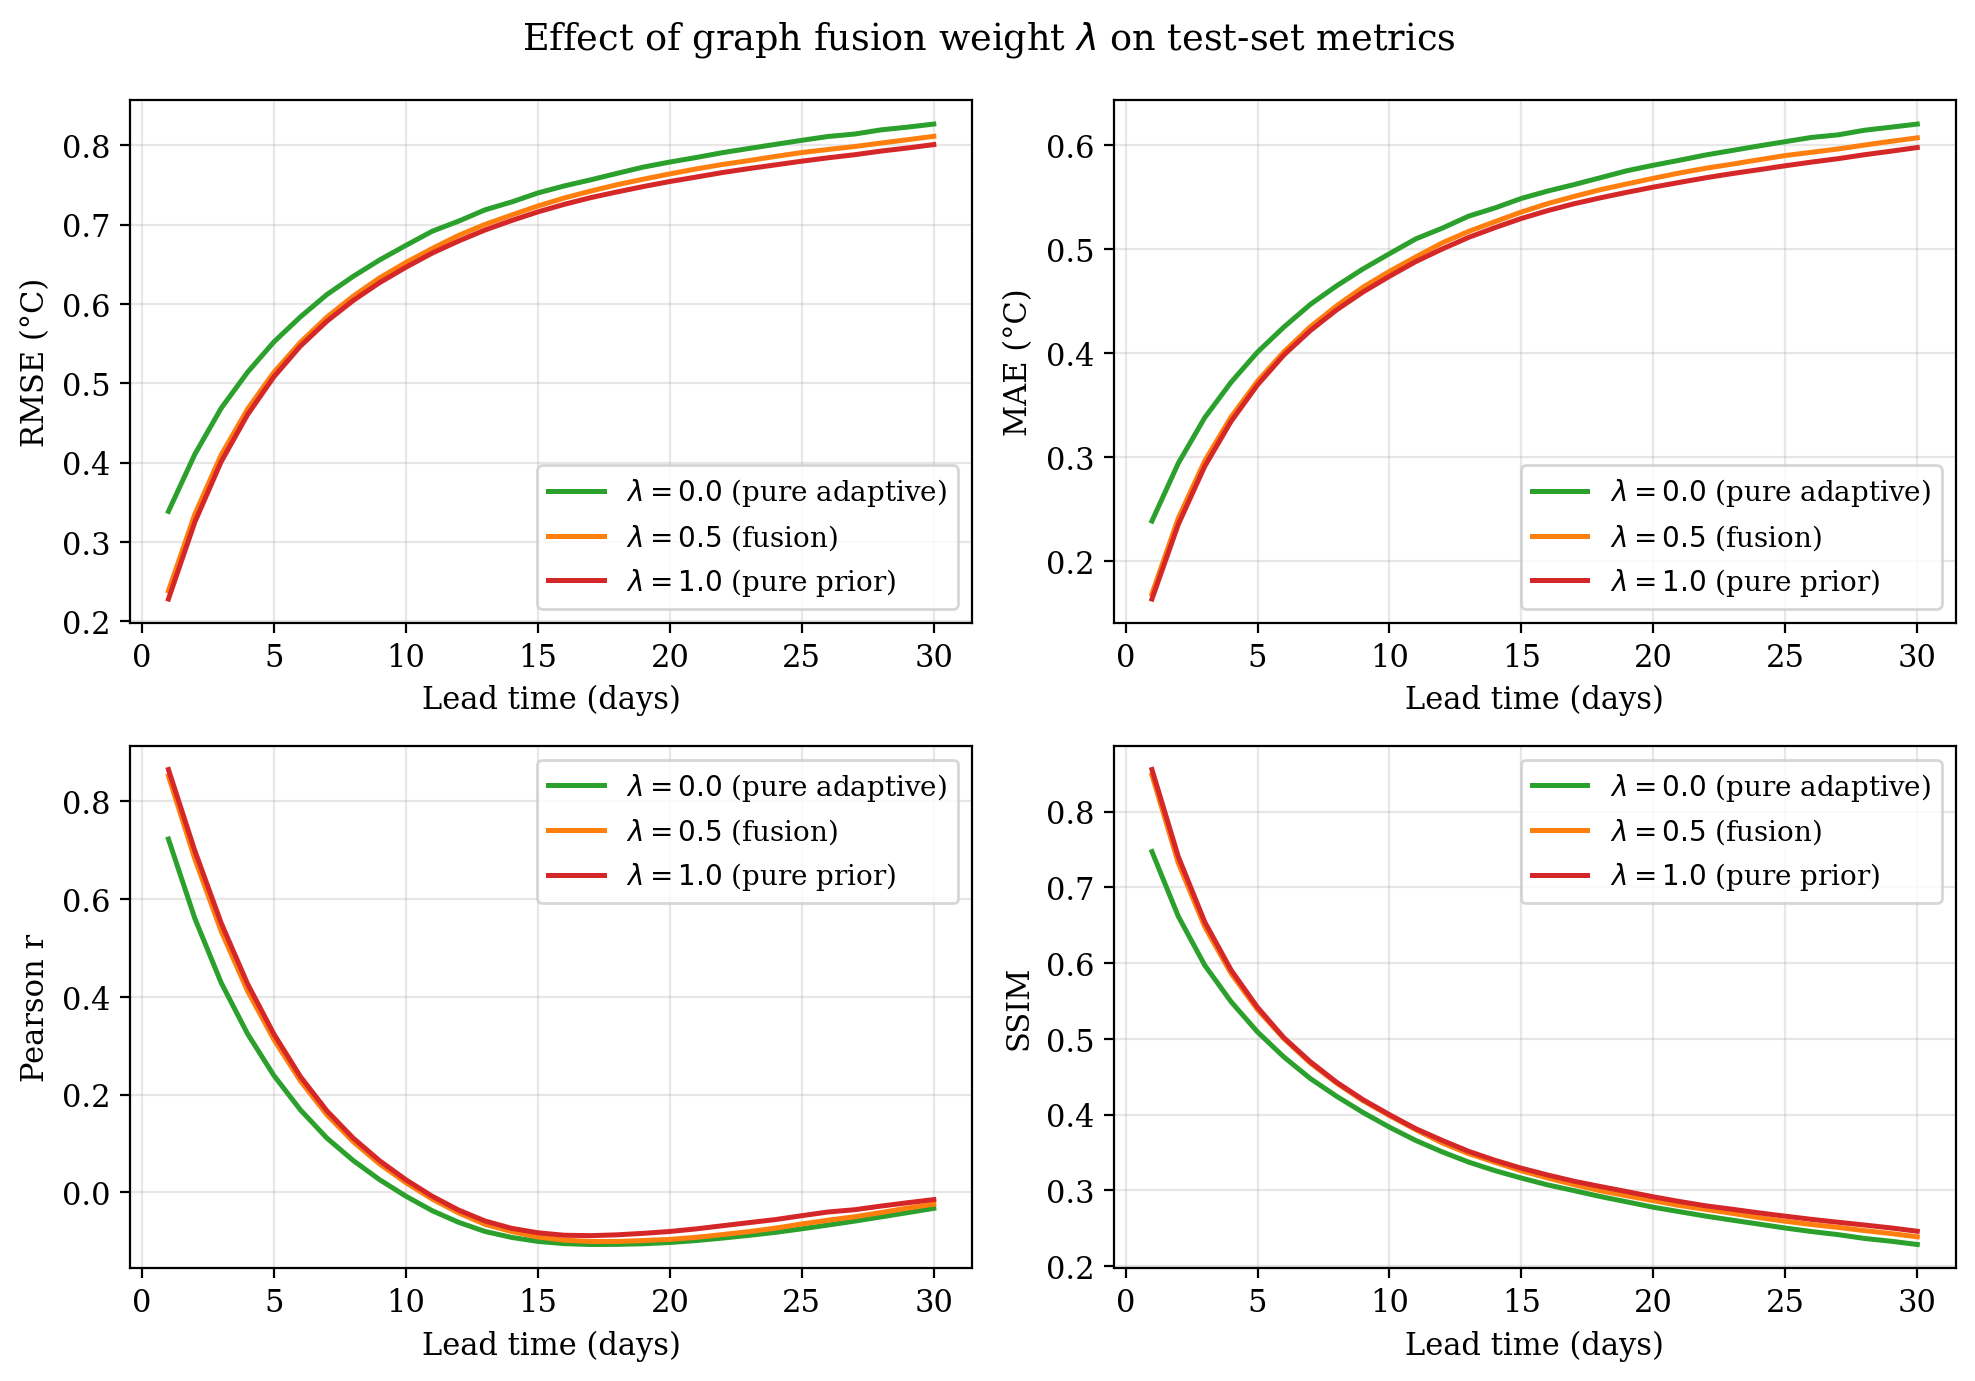
\includegraphics[width=0.95\linewidth]{figures/fig_lead_decay_ablation.png}
\caption{$\lambda$ 消融实验在全 30 天 lead 上的 RMSE / MAE / Pearson / SSIM 衰减曲线。}
\label{fig:lead_decay_ablation}
\end{figure}

\paragraph{结论 1：先验图是性能的主要来源。}
$\lambda=0$（纯自适应图）在所有 lead、所有指标上均显著劣于另外两组——尤其在 lead = 1 天 RMSE 上高出 $0.10\,^{\circ}$C 以上，相对偏差达 $48\%$。这说明在本任务的"高维空间 (N=2276)、小时序样本 ($\sim\!2.5$\,k 训练窗) 、弱监督 (仅末端重建误差)"组合下，自适应嵌入难以稳定地学到合理的图拓扑，反而引入显著噪声。

\paragraph{结论 2：等权融合带来最优验证集，但测试集略输于纯先验。}
$\lambda=0.5$ 取得最低验证集 RMSE (0.6668)，但其在测试集 4 个 lead RMSE 上均比 $\lambda=1.0$ 高 $0.005$\,--\,$0.011\,^{\circ}$C。这种"验证最优、测试稍差"是经典的轻度过拟合特征：自适应分支在验证集上拟合到了一定的伪相关结构，但在分布稍有漂移的测试集上未能泛化。

\paragraph{结论 3：基于地理距离的先验图近乎已是局部最优空间算子。}
SST 异常在大尺度上由平流--扩散主导，其支配方程在数值离散后的稳定模板就是基于距离衰减的拉普拉斯算子。这一物理事实使得我们构建的先验图（高斯核 + KNN 稀疏化 + 海陆/极地修正）已逼近"在当前网格分辨率下的最优空间相互作用模板"，留给自适应分支的"残差结构"非常有限。

\paragraph{对自适应分支为何失效的进一步讨论。}
AGCRN 的自适应邻接经由节点嵌入 $\boldsymbol{E}\in\mathbb{R}^{N\times d}$ 的内积重构：$\boldsymbol{A}_{\text{adapt}} = \mathrm{softmax}(\mathrm{ReLU}(\boldsymbol{E}\boldsymbol{E}^{\top}))$。仅 $\boldsymbol{E}$ 即包含 $N\!\times\!d = 2276\!\times\!10 \approx 2.3\!\times\!10^{4}$ 个可训练参数。然而其唯一监督信号来源于下游 30 天预测误差，对图结构的约束极弱。在样本量与隐式监督强度不匹配的设定下，自适应分支主要"消耗"模型容量而未带来增益。该现象与 \citet{shang2021dgsl, wang2023nograph} 所报告的"在中小数据集上学到的图常退化为类全连接或类噪声结构"是一致的。

% ---------------------------------------------------------------------
\section{综合讨论与局限}
\label{sec:exp:discussion}

\paragraph{所提方法的核心结论}
（1）在 SSTA 中长期预测任务上，AGCRN 较 Persistence/Climatology 取得稳定且统计上有意义的 RMSE 降低（$5.9\%$\,--\,$28.2\%$，依 lead 而异），证明所提"时空图神经网络 + 先验距离图"框架的有效性；
（2）模型最显著的优势区间出现在 lead 为 5\,--\,15 天的中期预测，对应 SSTA 任务的"动力可预测性窗口"；
（3）通过 $\lambda$ 消融发现：在当前数据规模下，由地理先验提供的固定图拓扑已近似最优，等权融合带来轻度过拟合，纯先验给出最佳测试性能。

\paragraph{当前局限}
（1）\textbf{数据规模}：训练窗口仅 $\sim\!2.5$\,k 个，不足以让 22\,k 维节点嵌入收敛——这是消融实验中自适应分支失效的根本原因。后续可通过将研究区域扩展到全球或加入历史更长的卫星 SST 数据集 (HadISST, ERSSTv5) 缓解。
（2）\textbf{评价的统计显著性}：本章主要结果基于单一随机种子的训练。$\lambda=0.5$ 与 $\lambda=1.0$ 在测试 RMSE 上的差距 ($\sim\!0.005$\,--\,$0.026\,^{\circ}$C) 接近 seed 间的训练噪声水平。需通过多 seed 重复实验对该结论进行配对显著性检验，相关结果将在附录中给出。
（3）\textbf{长期可预测性}：lead $\ge\!15$ 天时所有方法 Pearson $r$ 均落入 $[-0.1, 0]$ 区间，模型在该尺度仅"压缩幅值"而无法保持空间形状。突破该上限需引入大气强迫（风应力、热通量）或全球低频变率 (ENSO/PDO 指数) 等外部协变量，超出本工作的研究范围。
（4）\textbf{融合方式的简单性}：当前 $\lambda$ 为全局标量。若自适应分支仅在某些区域 (如 ENSO 区) 携带额外信息，则线性整图融合无法选择性激活该信号。后续可探索逐节点 / 逐区域门控融合 $\boldsymbol{A}_{\text{used}} = \boldsymbol{g}\odot\boldsymbol{A}_{\text{prior}} + (\mathbf{1}-\boldsymbol{g})\odot\boldsymbol{A}_{\text{adapt}}$，让模型自适应决定信任程度。
\end{document}
